\documentclass[10pt,a4paper,onecolumn]{article}
\usepackage{marginnote}
\usepackage{graphicx}
\usepackage{xcolor}
\usepackage{authblk,etoolbox}
\usepackage{titlesec}
\usepackage{calc}
\usepackage{tikz}
\usepackage{hyperref}
\hypersetup{colorlinks,breaklinks,
            urlcolor=[rgb]{0.0, 0.5, 1.0},
            linkcolor=[rgb]{0.0, 0.5, 1.0}}
\usepackage{caption}
\usepackage{tcolorbox}
\usepackage{amssymb,amsmath}
\usepackage{ifxetex,ifluatex}
\usepackage{seqsplit}
\usepackage{fixltx2e} % provides \textsubscript
\usepackage[
  backend=biber,
%  style=alphabetic,
%  citestyle=numeric
]{biblatex}
\bibliography{ms\_refs.bib}



% --- Page layout -------------------------------------------------------------
\usepackage[top=3.5cm, bottom=3cm, right=1.5cm, left=1.0cm,
            headheight=2.2cm, reversemp, includemp, marginparwidth=4.5cm]{geometry}

% --- Default font ------------------------------------------------------------
% \renewcommand\familydefault{\sfdefault}

% --- Style -------------------------------------------------------------------
\renewcommand{\bibfont}{\small \sffamily}
\renewcommand{\captionfont}{\small\sffamily}
\renewcommand{\captionlabelfont}{\bfseries}

% --- Section/SubSection/SubSubSection ----------------------------------------
\titleformat{\section}
  {\normalfont\sffamily\Large\bfseries}
  {}{0pt}{}
\titleformat{\subsection}
  {\normalfont\sffamily\large\bfseries}
  {}{0pt}{}
\titleformat{\subsubsection}
  {\normalfont\sffamily\bfseries}
  {}{0pt}{}
\titleformat*{\paragraph}
  {\sffamily\normalsize}


% --- Header / Footer ---------------------------------------------------------
\usepackage{fancyhdr}
\pagestyle{fancy}
\fancyhf{}
%\renewcommand{\headrulewidth}{0.50pt}
\renewcommand{\headrulewidth}{0pt}
\fancyhead[L]{\hspace{-0.75cm}\includegraphics[width=5.5cm]{/Library/Frameworks/R.framework/Versions/4.4-arm64/Resources/library/rticles/rmarkdown/templates/joss/resources/JOSS-logo.png}}
\fancyhead[C]{}
\fancyhead[R]{}
\renewcommand{\footrulewidth}{0.25pt}

\fancyfoot[L]{\footnotesize{\sffamily Sparks et al., (2025). hatchR: A
toolset to predict hatch and emergence phenology in wild
fishes. \textit{Journal of Open Source Software}, (), . \href{https://doi.org/}{https://doi.org/}}}


\fancyfoot[R]{\sffamily \thepage}
\makeatletter
\let\ps@plain\ps@fancy
\fancyheadoffset[L]{4.5cm}
\fancyfootoffset[L]{4.5cm}

% --- Macros ---------

\definecolor{linky}{rgb}{0.0, 0.5, 1.0}

\newtcolorbox{repobox}
   {colback=red, colframe=red!75!black,
     boxrule=0.5pt, arc=2pt, left=6pt, right=6pt, top=3pt, bottom=3pt}

\newcommand{\ExternalLink}{%
   \tikz[x=1.2ex, y=1.2ex, baseline=-0.05ex]{%
       \begin{scope}[x=1ex, y=1ex]
           \clip (-0.1,-0.1)
               --++ (-0, 1.2)
               --++ (0.6, 0)
               --++ (0, -0.6)
               --++ (0.6, 0)
               --++ (0, -1);
           \path[draw,
               line width = 0.5,
               rounded corners=0.5]
               (0,0) rectangle (1,1);
       \end{scope}
       \path[draw, line width = 0.5] (0.5, 0.5)
           -- (1, 1);
       \path[draw, line width = 0.5] (0.6, 1)
           -- (1, 1) -- (1, 0.6);
       }
   }

% --- Title / Authors ---------------------------------------------------------
% patch \maketitle so that it doesn't center
\patchcmd{\@maketitle}{center}{flushleft}{}{}
\patchcmd{\@maketitle}{center}{flushleft}{}{}
% patch \maketitle so that the font size for the title is normal
\patchcmd{\@maketitle}{\LARGE}{\LARGE\sffamily}{}{}
% patch the patch by authblk so that the author block is flush left
\def\maketitle{{%
  \renewenvironment{tabular}[2][]
    {\begin{flushleft}}
    {\end{flushleft}}
  \AB@maketitle}}
\makeatletter
\renewcommand\AB@affilsepx{ \protect\Affilfont}
%\renewcommand\AB@affilnote[1]{{\bfseries #1}\hspace{2pt}}
\renewcommand\AB@affilnote[1]{{\bfseries #1}\hspace{3pt}}
\makeatother
\renewcommand\Authfont{\sffamily\bfseries}
\renewcommand\Affilfont{\sffamily\small\mdseries}
\setlength{\affilsep}{1em}


\ifnum 0\ifxetex 1\fi\ifluatex 1\fi=0 % if pdftex
  \usepackage[T1]{fontenc}
  \usepackage[utf8]{inputenc}

\else % if luatex or xelatex
  \ifxetex
    \usepackage{mathspec}
  \else
    \usepackage{fontspec}
  \fi
  \defaultfontfeatures{Ligatures=TeX,Scale=MatchLowercase}

\fi
% use upquote if available, for straight quotes in verbatim environments
\IfFileExists{upquote.sty}{\usepackage{upquote}}{}
% use microtype if available
\IfFileExists{microtype.sty}{%
\usepackage{microtype}
\UseMicrotypeSet[protrusion]{basicmath} % disable protrusion for tt fonts
}{}

\usepackage{hyperref}
\hypersetup{unicode=true,
            pdftitle={hatchR: A toolset to predict hatch and emergence phenology in wild fishes},
            pdfborder={0 0 0},
            breaklinks=true}
\urlstyle{same}  % don't use monospace font for urls
\usepackage{graphicx,grffile}
\makeatletter
\def\maxwidth{\ifdim\Gin@nat@width>\linewidth\linewidth\else\Gin@nat@width\fi}
\def\maxheight{\ifdim\Gin@nat@height>\textheight\textheight\else\Gin@nat@height\fi}
\makeatother
% Scale images if necessary, so that they will not overflow the page
% margins by default, and it is still possible to overwrite the defaults
% using explicit options in \includegraphics[width, height, ...]{}
\setkeys{Gin}{width=\maxwidth,height=\maxheight,keepaspectratio}
\IfFileExists{parskip.sty}{%
\usepackage{parskip}
}{% else
\setlength{\parindent}{0pt}
\setlength{\parskip}{6pt plus 2pt minus 1pt}
}
\setlength{\emergencystretch}{3em}  % prevent overfull lines
\setcounter{secnumdepth}{0}
% Redefines (sub)paragraphs to behave more like sections
\ifx\paragraph\undefined\else
\let\oldparagraph\paragraph
\renewcommand{\paragraph}[1]{\oldparagraph{#1}\mbox{}}
\fi
\ifx\subparagraph\undefined\else
\let\oldsubparagraph\subparagraph
\renewcommand{\subparagraph}[1]{\oldsubparagraph{#1}\mbox{}}
\fi

% Pandoc syntax highlighting
\usepackage{color}
\usepackage{fancyvrb}
\newcommand{\VerbBar}{|}
\newcommand{\VERB}{\Verb[commandchars=\\\{\}]}
\DefineVerbatimEnvironment{Highlighting}{Verbatim}{commandchars=\\\{\}}
% Add ',fontsize=\small' for more characters per line
\usepackage{framed}
\definecolor{shadecolor}{RGB}{248,248,248}
\newenvironment{Shaded}{\begin{snugshade}}{\end{snugshade}}
\newcommand{\AlertTok}[1]{\textcolor[rgb]{0.94,0.16,0.16}{#1}}
\newcommand{\AnnotationTok}[1]{\textcolor[rgb]{0.56,0.35,0.01}{\textbf{\textit{#1}}}}
\newcommand{\AttributeTok}[1]{\textcolor[rgb]{0.13,0.29,0.53}{#1}}
\newcommand{\BaseNTok}[1]{\textcolor[rgb]{0.00,0.00,0.81}{#1}}
\newcommand{\BuiltInTok}[1]{#1}
\newcommand{\CharTok}[1]{\textcolor[rgb]{0.31,0.60,0.02}{#1}}
\newcommand{\CommentTok}[1]{\textcolor[rgb]{0.56,0.35,0.01}{\textit{#1}}}
\newcommand{\CommentVarTok}[1]{\textcolor[rgb]{0.56,0.35,0.01}{\textbf{\textit{#1}}}}
\newcommand{\ConstantTok}[1]{\textcolor[rgb]{0.56,0.35,0.01}{#1}}
\newcommand{\ControlFlowTok}[1]{\textcolor[rgb]{0.13,0.29,0.53}{\textbf{#1}}}
\newcommand{\DataTypeTok}[1]{\textcolor[rgb]{0.13,0.29,0.53}{#1}}
\newcommand{\DecValTok}[1]{\textcolor[rgb]{0.00,0.00,0.81}{#1}}
\newcommand{\DocumentationTok}[1]{\textcolor[rgb]{0.56,0.35,0.01}{\textbf{\textit{#1}}}}
\newcommand{\ErrorTok}[1]{\textcolor[rgb]{0.64,0.00,0.00}{\textbf{#1}}}
\newcommand{\ExtensionTok}[1]{#1}
\newcommand{\FloatTok}[1]{\textcolor[rgb]{0.00,0.00,0.81}{#1}}
\newcommand{\FunctionTok}[1]{\textcolor[rgb]{0.13,0.29,0.53}{\textbf{#1}}}
\newcommand{\ImportTok}[1]{#1}
\newcommand{\InformationTok}[1]{\textcolor[rgb]{0.56,0.35,0.01}{\textbf{\textit{#1}}}}
\newcommand{\KeywordTok}[1]{\textcolor[rgb]{0.13,0.29,0.53}{\textbf{#1}}}
\newcommand{\NormalTok}[1]{#1}
\newcommand{\OperatorTok}[1]{\textcolor[rgb]{0.81,0.36,0.00}{\textbf{#1}}}
\newcommand{\OtherTok}[1]{\textcolor[rgb]{0.56,0.35,0.01}{#1}}
\newcommand{\PreprocessorTok}[1]{\textcolor[rgb]{0.56,0.35,0.01}{\textit{#1}}}
\newcommand{\RegionMarkerTok}[1]{#1}
\newcommand{\SpecialCharTok}[1]{\textcolor[rgb]{0.81,0.36,0.00}{\textbf{#1}}}
\newcommand{\SpecialStringTok}[1]{\textcolor[rgb]{0.31,0.60,0.02}{#1}}
\newcommand{\StringTok}[1]{\textcolor[rgb]{0.31,0.60,0.02}{#1}}
\newcommand{\VariableTok}[1]{\textcolor[rgb]{0.00,0.00,0.00}{#1}}
\newcommand{\VerbatimStringTok}[1]{\textcolor[rgb]{0.31,0.60,0.02}{#1}}
\newcommand{\WarningTok}[1]{\textcolor[rgb]{0.56,0.35,0.01}{\textbf{\textit{#1}}}}

% tightlist command for lists without linebreak
\providecommand{\tightlist}{%
  \setlength{\itemsep}{0pt}\setlength{\parskip}{0pt}}

% From pandoc table feature
\usepackage{longtable,booktabs,array}
\usepackage{calc} % for calculating minipage widths
% Correct order of tables after \paragraph or \subparagraph
\usepackage{etoolbox}
\makeatletter
\patchcmd\longtable{\par}{\if@noskipsec\mbox{}\fi\par}{}{}
\makeatother
% Allow footnotes in longtable head/foot
\IfFileExists{footnotehyper.sty}{\usepackage{footnotehyper}}{\usepackage{footnote}}
\makesavenoteenv{longtable}

% Pandoc citation processing
%From Pandoc 3.1.8
% definitions for citeproc citations
\NewDocumentCommand\citeproctext{}{}
\NewDocumentCommand\citeproc{mm}{%
  \begingroup\def\citeproctext{#2}\cite{#1}\endgroup}
\makeatletter
 % allow citations to break across lines
 \let\@cite@ofmt\@firstofone
 % avoid brackets around text for \cite:
 \def\@biblabel#1{}
 \def\@cite#1#2{{#1\if@tempswa , #2\fi}}
\makeatother
\newlength{\cslhangindent}
\setlength{\cslhangindent}{1.5em}
\newlength{\csllabelwidth}
\setlength{\csllabelwidth}{3em}
\newenvironment{CSLReferences}[2] % #1 hanging-indent, #2 entry-spacing
 {\begin{list}{}{%
  \setlength{\itemindent}{0pt}
  \setlength{\leftmargin}{0pt}
  \setlength{\parsep}{0pt}
  % turn on hanging indent if param 1 is 1
  \ifodd #1
   \setlength{\leftmargin}{\cslhangindent}
   \setlength{\itemindent}{-1\cslhangindent}
  \fi
  % set entry spacing
  \setlength{\itemsep}{#2\baselineskip}}}
 {\end{list}}
\usepackage{calc}
\newcommand{\CSLBlock}[1]{#1\hfill\break}
\newcommand{\CSLLeftMargin}[1]{\parbox[t]{\csllabelwidth}{#1}}
\newcommand{\CSLRightInline}[1]{\parbox[t]{\linewidth - \csllabelwidth}{#1}\break}
\newcommand{\CSLIndent}[1]{\hspace{\cslhangindent}#1}



\title{hatchR: A toolset to predict hatch and emergence phenology in
wild fishes}

        \author[1]{Morgan M. Sparks}
          \author[2]{Eli Felts}
          \author[1]{Bryan M. Maitland}
    
      \affil[1]{US Forest Service, Rocky Mountain Research Station,
Boise, ID, USA}
      \affil[2]{US Fish and Wildlife Service, Idaho Fish and Wildlife
Conservation Office, Orofino, ID, USA}
  \date{\vspace{-5ex}}

\begin{document}
\maketitle

\marginpar{
  %\hrule
  \sffamily\small

  {\bfseries DOI:} \href{https://doi.org/}{\color{linky}{}}

  \vspace{2mm}

  {\bfseries Software}
  \begin{itemize}
    \setlength\itemsep{0em}
    \item \href{}{\color{linky}{Review}} \ExternalLink
    \item \href{}{\color{linky}{Repository}} \ExternalLink
    \item \href{}{\color{linky}{Archive}} \ExternalLink
  \end{itemize}

  \vspace{2mm}

  {\bfseries Submitted:} \\
  {\bfseries Published:} 

  \vspace{2mm}
  {\bfseries License}\\
  Authors of papers retain copyright and release the work under a Creative Commons Attribution 4.0 International License (\href{http://creativecommons.org/licenses/by/4.0/}{\color{linky}{CC-BY}}).
}

\section{Abstract}\label{abstract}

Understanding the timing of key life history events is necessary for
managing and conserving populations. Historically, models to predict
hatch and emergence timing for fishes were difficult to employ in wild
settings because average incubation temperature was needed as the
primary parameter in predictive models. However, recent improvements to
these techniques reworked models such that they could be applied in wild
environments as long as users had data for when adult fish spawned and a
record of average daily temperature over the course of development.
Despite these improvements, their application remains limited due to few
parameterizations for varying species, being largely limited to
salmonids. Here we present \textbf{hatchR}, a software ecosystem that
allows users to predict hatch and emergence timing for wild fishes, as
well as additional tools to aid in those analyses. \textbf{hatchR}
allows users to leverage popular historic parameterizations for
phenological models or to easily implement custom parameterizations
using data not included in the package. \textbf{hatchR} is also
distributed in two forms---an open source R package for maximum
customization, as well as an HTML graphical-user-interface web
application for individuals not familiar with scripting languages. To
demonstrate potential uses, we present two case studies as likely
applications for this software. \textbf{hatchR} promises to open many
exciting avenues in research and management of fishes during their early
life history.

\section{Introduction}\label{introduction}

As primarily poikilothermic organisms, the development and growth of
fishes is tightly linked with the temperature of their ambient
environment. This close relationship has allowed researchers to generate
statistical models that allow the prediction of developmental phenology
with high accuracy and precision. These models were typically developed
in aquaculture settings and their initial formulations were not
applicable to wild populations because they assumed a constant
temperature over the course of development (Alderdice \& Velsen, 1978;
Beacham \& Murray, 1990; McPhail \& Murray, 1979). However, Sparks et
al. (2019) reformulated this approach as an ``Effective Value model'',
in which the input was daily average temperature after a parent spawned
and fish would either hatch or emerge when effective values cumulatively
summed to one.

The resulting effective value approach has now been widely applied in
Salmonids for which parameterizations from aquaculture were readily
available---for example Pacific Salmon (\emph{Oncorhynchus spp.}) models
developed by Beacham \& Murray (1990) have been applied to various
species and populations (Adelfio, Wondzell, Mantua, \& Reeves, 2019,
2024; Kaylor et al., 2021) while models developed for Bull Trout
(\emph{Salvelinus confluentus}) by McPhail \& Murray (1979) were
extended by Austin, Essington, \& Quinn (2019). Despite growing
popularity, applications have been largely limited within Salmonids,
presumably because parameterizations for such models already existed due
to their wide use in aquaculture and their general popularity as sport
and commercial fish.

To bridge the gap between the application of one-off effective value
model applications within individual studies and the lack of
parameterization for other species, we developed the software ecosystem,
\textbf{hatchR}. Specifically, \textbf{hatchR} allows users to input
standard raw or summarized temperature datasets that are commonly
collected in wild settings, run basic checks on those data, use built-in
parameterizations like those from Beacham \& Murray (1990) or Sparks,
Westley, Falke, \& Quinn (2017), develop custom models from their own or
published temperature and phenological data, and predict hatch and
emergence timing using these models in the effective value framework.

To widen the user application of these methods, we distribute two
user-interfaces for \textbf{hatchR}. The first is a R package ({``R''}
(n.d.)) distributed via CRAN that allows users the most customizable
application for these methods. The R package is especially powerful as
it allows users to automate their analyses over multiple variables such
as phenology type, multiple spawn dates, or different habitats with
varying thermal regimes. These variable approaches are outlined in the
package documentation on \textbf{hatchR}'s website. Alternatively, we
also distribute a Shiny application (Chang et al. (2024)) in the form of
an HTML-based web tool to interact with many of \textbf{hatchR}'s
functions in a graphical-user-interface. The Shiny form trades-off some
of automative power for user simplicity, while still allowing users to
leverage much of the functionality of \textbf{hatchR}'s R package.
Below, we present the basic overview of the software and multiple case
studies of how it may be applied.

\section{Package Overview}\label{package-overview}

\textbf{hatchR} is meant to primarily be a tool for predicting
phenology. In this sense, we limit functionality to these applications
and provide minimal data checking and plotting help. This decision is in
part driven by the diversity of data types that users may import and the
difficulty in addressing all those data types with respect to various
data checks. In other words, we expect users to know their data better
than we do and to check it accordingly. We do provide two basic data
check functions discussed in the Checking Data section. Similarly, we
provide limited functionality for plotting results, but provide examples
of how to build custom visualizations from output, specifically in R.
For the Shiny application, we provide a base output plot, but the
ability to download your results for custom plotting in programs of the
user's choice. Finally, we provide brief summaries of general
applications of \textbf{hatchR} below, but encourage users to visit
articles hosted on the software webpage that extensively outline primary
functions and applications, especially automating the application of
predicting phenology across multiple variables.

\begin{figure}

{\centering 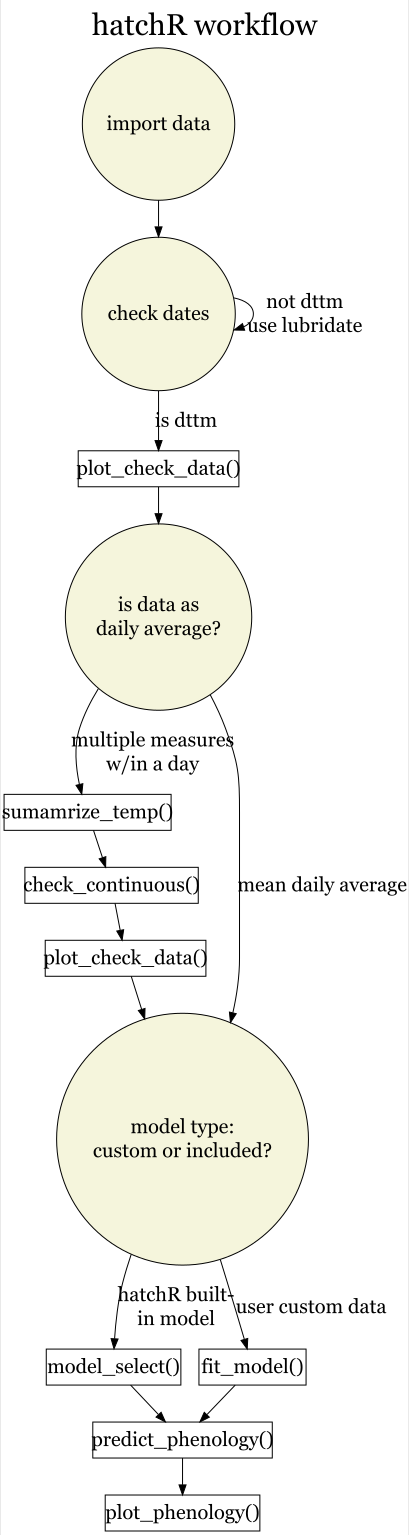
\includegraphics[width=5.68in,height=0.5\textheight]{flowchart} 

}

\caption{Full workflow for hatchR. Data processes are demonstrated with beige circles and pakcage functions with white rectangles.}\label{fig:unnamed-chunk-3}
\end{figure}

\subsection{Effective value models}\label{effective-value-models}

Effective value models were created by Sparks et al. (2019) to implement
developmental models in wild environments for Sockeye Salmon (\emph{O.
nerka}). The need for their development arose because historic models,
specifically those in Beacham \& Murray (1990), only considered the
average incubation temperature during development and, for wild fishes,
average incubation temperature was impossible to estimate because it was
unknown when fish hatched even if adult spawn timing was known. To
address this, Sparks et al. (2019) used the reciprocal of the
formulation of model 2 from Beacham \& Murray (1990) and assigned an
effective value for every day of development using the daily average
temperature.

The model follows the general format of:

\[
Effective Value_i = 1/exp(log_ea - log_e(Temperature_i - b))
\]

Where \emph{i} is the daily value and a fish hatches or emerges when the
cumulative sum of effective values reaches one:
\[\sum_{i =1}^nEffectiveValue_i = 1\]

The effective value model framework is the basis for the phenological
models in \textbf{hatchR}, both in the included \texttt{model\_table} in
the package (though \texttt{model\_table} includes more complex models
developed by Beacham \& Murray (1990)), as well as for custom models
users can fit with \texttt{fit\_model()}. Specifically,
\texttt{model\_table} includes parameterizations from Beacham \& Murray
(1990), Sparks et al. (2017), and Austin et al. (2019) (who extended
McPhail \& Murray (1979)).

\subsection{Data format}\label{data-format}

Water temperature datasets collected for wild environments are often
either 1.) already summarized by day (\emph{i.e.}, mean daily
temperature) or, 2.) in a raw format from something like a HOBO TidbiT
where readings are taken multiple times per day, which can be summarized
into a mean daily temperatures. Alternatively, new statistical models
like that of Siegel, Fullerton, FitzGerald, Holzer, \& Jordan (2023)
could be similarly implemented.

Fundamentally, \textbf{hatchR} assumes you have input data with two
columns: a date column, giving the date (and often time) of a
temperature measurement, and a temperature column, giving the associated
temperature measurement (in centigrade). Other columns are okay to
include, but these two columns (with any column name---just
\emph{without} spaces) are required. We expect your data to look
something like this:

\begin{longtable}[]{@{}ll@{}}
\toprule\noalign{}
date & temperature \\
\midrule\noalign{}
\endhead
\bottomrule\noalign{}
\endlastfoot
2000-01-01 & 2.51 \\
\ldots{} & \ldots{} \\
2000-07-01 & 16.32 \\
\ldots{} & \ldots{} \\
2000-12-31 & 3.13 \\
\end{longtable}

\textbf{hatchR} assumes you've checked for missing records or errors in
your data as it \emph{will function with gaps}, so it's important to go
through the data checks discussed below, as well as your own validity
checks. \textbf{hatchR} can use values down to freezing (e.g, 0 °C),
which returns extremely small effective values, and time to hatch or
emerge may be \textgreater{} 1 year. In these cases, we suggest users
consider how much of that data type is reasonable with their data.

For users choosing to implement \textbf{hatchR} in R, data can be
imported from any format the user chooses, as long as users can
eventually coerce their data into a \texttt{dataframe} or
\texttt{tibble} format, in which each row represents a single record.
For the Shiny application, users must have their data stored as a .csv
(comma separated values) file for upload, which can easily be exported
using datasheet software like Microsoft Excel or Google Sheets.

\subsection{Checking Data}\label{checking-data}

\textbf{hatchR} is built assuming data will be analyzed as daily average
temperatures. Despite that assumption, raw data (\emph{e.g.}, as
outputted by HOBO loggers) can be used and \textbf{hatchR} includes
functionality to summarize those data into a format that is usable (only
in R, it must be summarized for the Shiny app), as well as provides
functions for basic visual and programmatic data checks to make sure
outliers or missing data are at least brought to user's attention.

We demonstrate the utility of the summary and check functions
\texttt{summarize\_temp()}, \texttt{plot\_check\_temp()}, and
\texttt{check\_continuous()} using a simulated year-long dataset with
temperature readings every thirty minutes.

\begin{Shaded}
\begin{Highlighting}[]
\CommentTok{\# create date object for a year with 30 min reading intervals}
\NormalTok{dates }\OtherTok{\textless{}{-}} \FunctionTok{seq}\NormalTok{(}\AttributeTok{from =} \FunctionTok{ymd\_hms}\NormalTok{(}\StringTok{"2000{-}07{-}01 00:00:00"}\NormalTok{),}
             \AttributeTok{to =} \FunctionTok{ymd\_hms}\NormalTok{(}\StringTok{"2001{-}06{-}30 23:59:59"}\NormalTok{), }\AttributeTok{length.out =} \DecValTok{17568}\NormalTok{) }

\CommentTok{\# create empty dataframe}
\NormalTok{year\_sim }\OtherTok{\textless{}{-}} \FunctionTok{data.frame}\NormalTok{(}\FunctionTok{matrix}\NormalTok{(}\ConstantTok{NA}\NormalTok{, }\AttributeTok{nrow =} \FunctionTok{length}\NormalTok{(dates), }\AttributeTok{ncol =} \DecValTok{1}\NormalTok{)) }

\CommentTok{\# date column}
\FunctionTok{colnames}\NormalTok{(year\_sim)[}\DecValTok{1}\NormalTok{] }\OtherTok{\textless{}{-}} \StringTok{"date"} 

\CommentTok{\# add dates vector to date column}
\NormalTok{year\_sim[}\DecValTok{1}\NormalTok{] }\OtherTok{\textless{}{-}}\NormalTok{ dates }

\CommentTok{\#random seed}
\FunctionTok{set.seed}\NormalTok{(}\DecValTok{123}\NormalTok{)}

\CommentTok{\# take temps from a random normal dist with mean 10 sd 3 }
\CommentTok{\# for every date time combo in dates and append to column (temp) }
\CommentTok{\# in year\_sim}
\NormalTok{year\_sim}\SpecialCharTok{$}\NormalTok{temp }\OtherTok{\textless{}{-}} \FunctionTok{rnorm}\NormalTok{(}\AttributeTok{n =} \FunctionTok{length}\NormalTok{(dates), }\AttributeTok{mean =} \DecValTok{10}\NormalTok{, }\AttributeTok{sd =} \DecValTok{3}\NormalTok{) }\SpecialCharTok{\%\textgreater{}\%}
  \FunctionTok{abs}\NormalTok{() }

\FunctionTok{dim}\NormalTok{(year\_sim)}
\end{Highlighting}
\end{Shaded}

\begin{verbatim}
## [1] 17568     2
\end{verbatim}

First, we recommend checking imported data for any outliers or strange
inputs using \texttt{plot\_check\_temp()}

\begin{Shaded}
\begin{Highlighting}[]
\FunctionTok{plot\_check\_temp}\NormalTok{(}\AttributeTok{data =}\NormalTok{ year\_sim,}
                \AttributeTok{dates =}\NormalTok{ date,}
                \AttributeTok{temperature =}\NormalTok{ temp,}
                \AttributeTok{temp\_min =} \DecValTok{0}\NormalTok{, }\CommentTok{\# temp\_min and max lines are }
                              \CommentTok{\# user customizable}
                \AttributeTok{temp\_max =} \DecValTok{25}\NormalTok{)}
\end{Highlighting}
\end{Shaded}

\begin{figure}
\centering
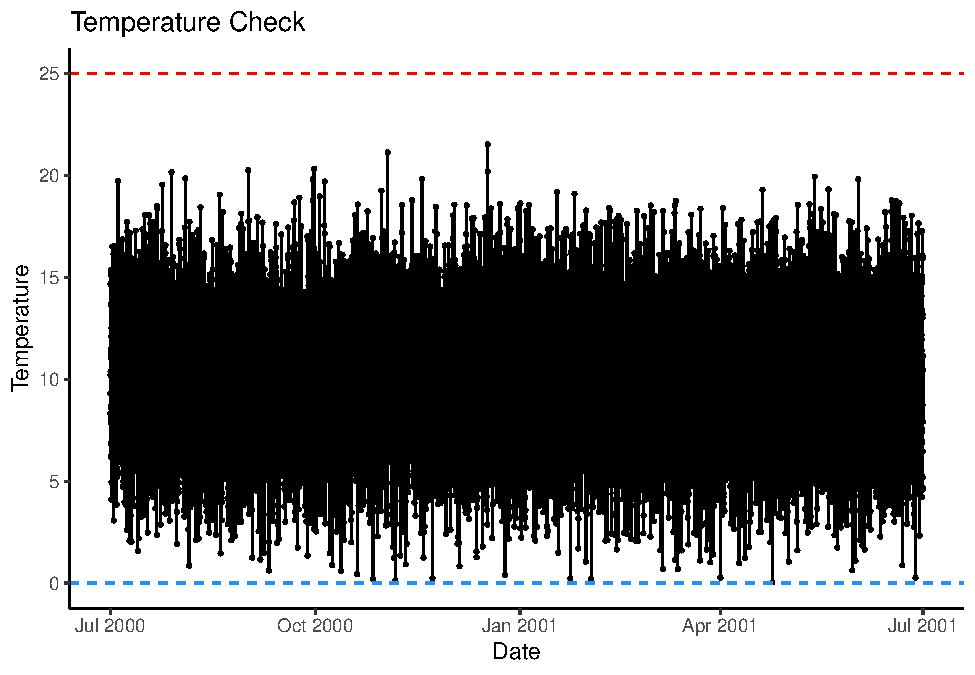
\includegraphics{paper_files/figure-latex/unnamed-chunk-5-1.pdf}
\caption{Full output of the plot\_check\_temp() visual data check
function from hatchR. Note that the red and blue lines are customizable
by the user to create outlier thresholds for their visual check.}
\end{figure}

There are no obvious outliers but since each day has 48 records, we need
to summarize it to daily mean temperature with
\texttt{summarize\_temp()} and then check for missing days with
\texttt{check\_continuous()}. We also recommend using
\texttt{plot\_check\_temp()} again on the summarized data (though leave
out the resulting plot for space efficiency in this manuscript).

\begin{Shaded}
\begin{Highlighting}[]
\CommentTok{\# summarize}
\NormalTok{year\_sim\_summ }\OtherTok{\textless{}{-}} \FunctionTok{summarize\_temp}\NormalTok{(}\AttributeTok{data =}\NormalTok{ year\_sim,}
                                \AttributeTok{dates =}\NormalTok{ date,}
                                \AttributeTok{temperature =}\NormalTok{ temp)}

\CommentTok{\# now a year\textquotesingle{}s worth of single{-}day data}
\FunctionTok{dim}\NormalTok{(year\_sim\_summ)}
\end{Highlighting}
\end{Shaded}

\begin{verbatim}
## [1] 365   2
\end{verbatim}

\begin{Shaded}
\begin{Highlighting}[]
\CommentTok{\# check continuous (no errors)}
\FunctionTok{check\_continuous}\NormalTok{(}\AttributeTok{data =}\NormalTok{ year\_sim\_summ,}
                 \AttributeTok{dates =}\NormalTok{ date)}
\end{Highlighting}
\end{Shaded}

\begin{verbatim}
## i No breaks were found. All clear!
\end{verbatim}

\begin{Shaded}
\begin{Highlighting}[]
\CommentTok{\# we can demonstrate an error by removing Oct. 8 (100th day)}
\FunctionTok{check\_continuous}\NormalTok{(}\AttributeTok{data =}\NormalTok{ year\_sim\_summ[}\SpecialCharTok{{-}}\DecValTok{100}\NormalTok{,],}
                 \AttributeTok{dates =}\NormalTok{ date)}
\end{Highlighting}
\end{Shaded}

\begin{verbatim}
## Warning: ! Data not continuous
## i Breaks found at rows:
## i 100
\end{verbatim}

\subsection{Model Selection}\label{model-selection}

Users can either use Salmonid models from \texttt{model\_table} included
in the package and the Shiny app. As discussed, these models are
included because parameterizations already existed in the literature.
However, these parameterizations are limited to Pacific Salmon and Bull
Trout. To widen the application of the effective value approach, we
include a \texttt{fit\_model()} function, which is species agnostic (as
long as development generally follows the power law).

The function \texttt{fit\_model()} uses data in which average incubation
temperature (°C) and days to phenological event (as two vectors) are the
inputs. The function estimates parameter coefficients for
\emph{log\textsubscript{e}a} and \emph{b} using \texttt{stats::nls()}

\textbf{BRYAN TO FINISH THIS PARAGRAPH OFF HERE}

\paragraph{Fitting models for other
fishes}\label{fitting-models-for-other-fishes}

Below, we demonstrate how the \texttt{fit\_model()} function may be used
to create custom parameterizations for species beyond the Salmonids in
the \texttt{model\_table} included in the package. We include
parameterizations from three warm-water species to demonstrate the
\texttt{fit\_model()} utility for fishes beyond the scope of the
original effective value approach. These parameterizations are for
commonly cultured sportfishes including Smallmouth Bass
(\emph{Micropterus dolomieu}) from Webster (1948), Channel Catfish
(\emph{Ictalurus punctatus}) from Small \& Bates (2001), and Lake
Sturgeon (\emph{Acipenser fulvescens}) from Smith \& King (2005). We
provide parameterization for just Smallmouth Bass here for concision,
but the full code set for all species is available at
\url{https://github.com/bmait101/hatchR/blob/master/inst/manuscript/paper.Rmd}.

We demonstrate the utility of this approach by creating a random thermal
regime with an ascending thermograph with a mean temperature of 16 °C,
parameterizing models for each species, and demonstrating days to hatch
and developmental period for each species with the random thermal regime
(Figure 3).

\begin{Shaded}
\begin{Highlighting}[]
\DocumentationTok{\#\#\#  make temp regime}
\FunctionTok{set.seed}\NormalTok{(}\DecValTok{123}\NormalTok{)}
\CommentTok{\# create random temps and corresponding dates}
\NormalTok{temps\_sim }\OtherTok{\textless{}{-}} \FunctionTok{sort}\NormalTok{(}\FunctionTok{rnorm}\NormalTok{(}\AttributeTok{n =}\DecValTok{30}\NormalTok{, }\AttributeTok{mean =} \DecValTok{16}\NormalTok{, }\AttributeTok{sd =} \DecValTok{1}\NormalTok{), }\AttributeTok{decreasing =} \ConstantTok{FALSE}\NormalTok{)}
\NormalTok{dates\_sim }\OtherTok{\textless{}{-}}  \FunctionTok{seq}\NormalTok{(}\AttributeTok{from =} \FunctionTok{ymd}\NormalTok{(}\StringTok{"2000{-}07{-}01"}\NormalTok{),}
             \AttributeTok{to =} \FunctionTok{ymd}\NormalTok{(}\StringTok{"2000{-}07{-}31"}\NormalTok{), }\AttributeTok{length.out =} \DecValTok{30}\NormalTok{)}

\NormalTok{data\_sim }\OtherTok{\textless{}{-}} \FunctionTok{matrix}\NormalTok{(}\ConstantTok{NA}\NormalTok{, }\DecValTok{30}\NormalTok{, }\DecValTok{2}\NormalTok{) }\SpecialCharTok{|\textgreater{}} \FunctionTok{data.frame}\NormalTok{()}
\NormalTok{data\_sim[,}\DecValTok{1}\NormalTok{] }\OtherTok{\textless{}{-}}\NormalTok{ temps\_sim}
\NormalTok{data\_sim[,}\DecValTok{2}\NormalTok{] }\OtherTok{\textless{}{-}}\NormalTok{ dates\_sim}

\CommentTok{\# change names so they aren\textquotesingle{}t the same as the vector objects}
\FunctionTok{colnames}\NormalTok{(data\_sim) }\OtherTok{\textless{}{-}} \FunctionTok{c}\NormalTok{(}\StringTok{"temp\_sim"}\NormalTok{, }\StringTok{"date\_sim"}\NormalTok{)}

\DocumentationTok{\#\#\# smallmouth mod}
\NormalTok{smallmouth }\OtherTok{\textless{}{-}} \FunctionTok{matrix}\NormalTok{(}\ConstantTok{NA}\NormalTok{, }\DecValTok{10}\NormalTok{, }\DecValTok{2}\NormalTok{) }\SpecialCharTok{|\textgreater{}} \FunctionTok{data.frame}\NormalTok{()}
\FunctionTok{colnames}\NormalTok{(smallmouth) }\OtherTok{\textless{}{-}} \FunctionTok{c}\NormalTok{(}\StringTok{"hours"}\NormalTok{, }\StringTok{"temp\_F"}\NormalTok{)}
\NormalTok{smallmouth}\SpecialCharTok{$}\NormalTok{hours }\OtherTok{\textless{}{-}} \FunctionTok{c}\NormalTok{(}\DecValTok{52}\NormalTok{, }\DecValTok{54}\NormalTok{, }\DecValTok{70}\NormalTok{, }\DecValTok{78}\NormalTok{, }\DecValTok{90}\NormalTok{, }\DecValTok{98}\NormalTok{, }\DecValTok{150}\NormalTok{, }\DecValTok{167}\NormalTok{, }\DecValTok{238}\NormalTok{, }\DecValTok{234}\NormalTok{)}
\NormalTok{smallmouth}\SpecialCharTok{$}\NormalTok{temp\_F }\OtherTok{\textless{}{-}} \FunctionTok{c}\NormalTok{(}\DecValTok{77}\NormalTok{, }\DecValTok{75}\NormalTok{, }\DecValTok{71}\NormalTok{, }\DecValTok{70}\NormalTok{, }\DecValTok{67}\NormalTok{, }\DecValTok{65}\NormalTok{, }\DecValTok{60}\NormalTok{, }\DecValTok{59}\NormalTok{, }\DecValTok{55}\NormalTok{, }\DecValTok{55}\NormalTok{)}

\CommentTok{\# change F to C and hours to days}
\NormalTok{smallmouth }\OtherTok{\textless{}{-}}\NormalTok{ smallmouth }\SpecialCharTok{|\textgreater{}} 
  \FunctionTok{mutate}\NormalTok{(}\AttributeTok{days =} \FunctionTok{ceiling}\NormalTok{(hours}\SpecialCharTok{/}\DecValTok{24}\NormalTok{),}
         \AttributeTok{temp\_C =}\NormalTok{ (temp\_F }\SpecialCharTok{{-}}\DecValTok{32}\NormalTok{) }\SpecialCharTok{*}\NormalTok{ (}\DecValTok{5}\SpecialCharTok{/}\DecValTok{9}\NormalTok{))}


\NormalTok{smb\_mod }\OtherTok{\textless{}{-}} \FunctionTok{fit\_model}\NormalTok{(}\AttributeTok{temp =}\NormalTok{ smallmouth}\SpecialCharTok{$}\NormalTok{temp\_C,}
                     \AttributeTok{days =}\NormalTok{ smallmouth}\SpecialCharTok{$}\NormalTok{days,}
                     \AttributeTok{species =} \StringTok{"smb"}\NormalTok{,}
                     \AttributeTok{development\_type =} \StringTok{"hatch"}\NormalTok{)}
\end{Highlighting}
\end{Shaded}

Note the \emph{R\textsuperscript{2}} fit from the models below. You can
see they generally all preform well and are in line with values from
model 2 of Beacham \& Murray (1990).

\begin{Shaded}
\begin{Highlighting}[]
\CommentTok{\#model fits}
\NormalTok{smb\_mod}\SpecialCharTok{$}\NormalTok{r\_squared; cat\_mod}\SpecialCharTok{$}\NormalTok{r\_squared; sturgeon\_mod}\SpecialCharTok{$}\NormalTok{r\_squared}
\end{Highlighting}
\end{Shaded}

\begin{verbatim}
## [1] 0.9868067
\end{verbatim}

\begin{verbatim}
## [1] 0.9433598
\end{verbatim}

\begin{verbatim}
## [1] 0.9217358
\end{verbatim}

\begin{figure}
\centering
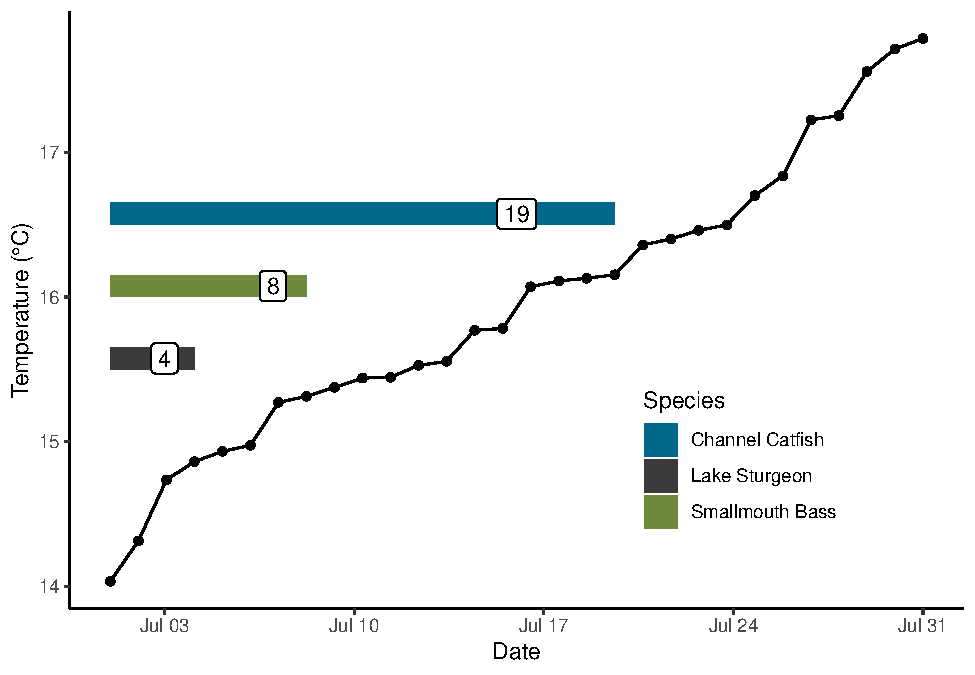
\includegraphics{paper_files/figure-latex/unnamed-chunk-10-1.pdf}
\caption{Days to hatch as predicted using custom parameterizations for
Channel Catfish (blue), Lake Sturgeon (black, and Smallmouth Bass
(green) as generated by the fit\_model() function in hathcR. Models are
all run using a spawn date starting June 1 for a randomly generated
ascending thermal regime with mean temperature 16 °C}
\end{figure}

\subsection{Predicting Phenology and
Output}\label{predicting-phenology-and-output}

To illustrate model selection and phenology prediction we will recreate
a small portion of the analysis done by Sparks et al. (2019) using the
\texttt{woody\_island} dataset included in this package . We will
predict both hatch and emergence timing, so we will obtain a model
expression for each using \texttt{model\_select()}.

\begin{Shaded}
\begin{Highlighting}[]
\NormalTok{sockeye\_hatch\_mod }\OtherTok{\textless{}{-}} \FunctionTok{model\_select}\NormalTok{(}
  \AttributeTok{author =} \StringTok{"Beacham and Murray 1990"}\NormalTok{, }
  \AttributeTok{species =} \StringTok{"sockeye"}\NormalTok{, }
  \AttributeTok{model =} \DecValTok{2}\NormalTok{, }
  \AttributeTok{development\_type =} \StringTok{"hatch"}
\NormalTok{  )}
\end{Highlighting}
\end{Shaded}

We can now use our model expressions to predict when sockeye would hatch
and emerge at Woody Island in 1990. First we predict hatch timing using
\texttt{predict\_phenology()}:

\begin{Shaded}
\begin{Highlighting}[]
\NormalTok{WI\_hatch }\OtherTok{\textless{}{-}} \FunctionTok{predict\_phenology}\NormalTok{(}
  \AttributeTok{data =}\NormalTok{ woody\_island,}
  \AttributeTok{dates =}\NormalTok{ date,}
  \AttributeTok{temperature =}\NormalTok{ temp\_c,}
  \AttributeTok{spawn.date =} \StringTok{"1990{-}08{-}18"}\NormalTok{,}
  \AttributeTok{model =}\NormalTok{ sockeye\_hatch\_mod}
\NormalTok{  )}
\end{Highlighting}
\end{Shaded}

And then look inside the returned object to see days to hatch and
development period:

\begin{Shaded}
\begin{Highlighting}[]
\NormalTok{WI\_hatch}\SpecialCharTok{$}\NormalTok{days2done}
\end{Highlighting}
\end{Shaded}

\begin{verbatim}
## NULL
\end{verbatim}

\begin{Shaded}
\begin{Highlighting}[]
\NormalTok{WI\_hatch}\SpecialCharTok{$}\NormalTok{dev.period}
\end{Highlighting}
\end{Shaded}

\begin{verbatim}
##        start       stop
## 1 1990-08-18 1990-10-30
\end{verbatim}

\paragraph{Understanding your results}\label{understanding-your-results}

The output from \texttt{predict\_phenology()} includes a lot of
information. If we look at our \texttt{WI\_hatch} object we see there
are multiple elements stored in a list which can be accessed using the
\texttt{\$} operator.

\begin{Shaded}
\begin{Highlighting}[]
\FunctionTok{str}\NormalTok{(WI\_hatch)}
\end{Highlighting}
\end{Shaded}

\texttt{WI\_hatch\$days2done} outputs the predicted days to develop.

\texttt{WI\_hatch\$dev.period} is a 1x2 dataframe with the dates
corresponding to when your fish's parent spawned (which you input with
\texttt{predict\_phenology(spawn.date\ =\ ...)}) and the date when the
fish is predicted todevelop.

\texttt{WI\_hatch\$ef.vals} is a vector of each day's effective value as
evaluated using whatever model is chosen.

\texttt{WI\_hatch\$ef.tibble} is a \emph{n} x 4 tibble (\emph{n} =
number of days to hatch or emerge) and the columns are the date, each
day's temperature and effective value, and the cumulative sum of the
effective values. The \texttt{ef.tibble} object is meant to serve as the
basis for users to make custom figures for their data beyond the
functionality we discuss below.

\paragraph{Plotting phenology}\label{plotting-phenology}

\textbf{hatchR} has a built in function, \texttt{plot\_phenology()},
that allows users to visualize their phenology results (Figure 4). The
plot visualizes three specific components: 1.) the temperature regime
over which you are predicting, 2.) the cumulative sum of effective
values, and 3.) the effective value for each day in your prediction
span. The function allows you to output various figures based on your
interests, but defaults to a figure with all information and the
corresponding labels.

\begin{Shaded}
\begin{Highlighting}[]
\FunctionTok{plot\_phenology}\NormalTok{(WI\_hatch)}
\end{Highlighting}
\end{Shaded}

\begin{figure}
\centering
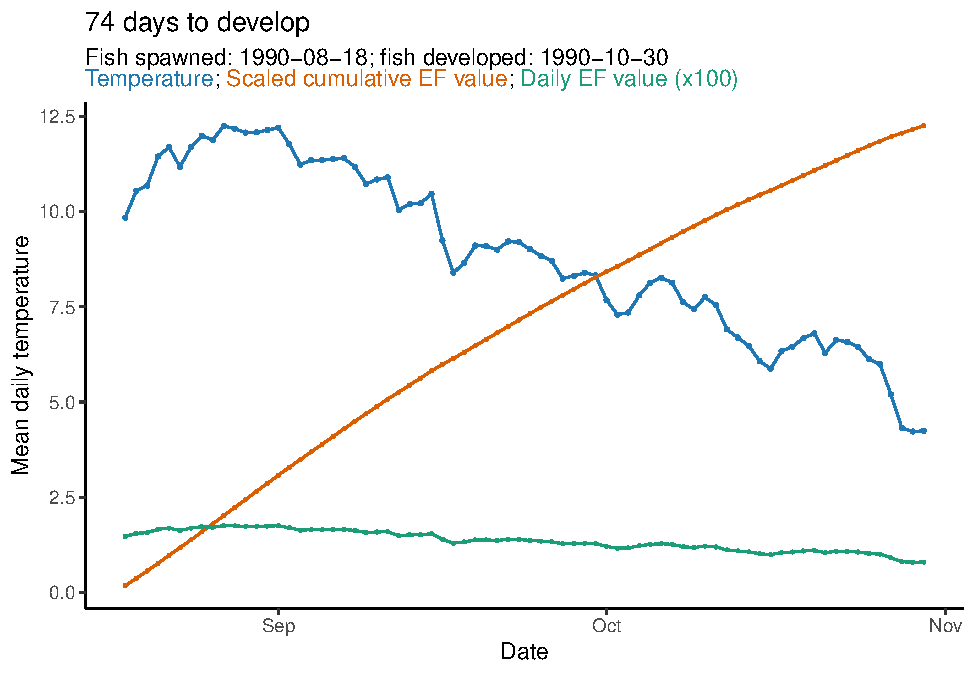
\includegraphics{paper_files/figure-latex/unnamed-chunk-15-1.pdf}
\caption{Output of the plot\_phenology() function from hatchR. The
function plots the output of the predict\_phenology() function and
displays time to develop, as well as the ambient thermal regime (blue),
scaled daily effective value (green), and the scaled cumulative sum of
effective values (orange).}
\end{figure}

\section{Case Study 1}\label{case-study-1}

A common management scenario where developmental phenology might be
useful would be trying to understand if fish might be free-moving before
some management action. For instance, will fish have emerged from redds
when a stream section has been opened to grazing or road work?

In this scenario, we will consider the road work example and Bull Trout,
a threatened fish in the United States under the Endangered Species Act
(Nolfi, Melbihess, Fisher, \& Ellis, 2024), and the Crooked River, a key
Bull Trout population in the Boise River watershed. In this hypothetical
scenario, the Forest Fisheries Biologist wants to know if fish will
likely be out of the gravel and free-swimming by June 1st as Bull Trout
are particularly sensitive to sediment. In this system, it is expected
that Bull Trout will be done spawning by the end of September, so we'll
consider the last possible spawn date as September 30th.

We demonstrate this first case study using the graphical user interface
portion of the \textbf{hatchR} ecosystem found at
\url{https://elifelts.shinyapps.io/hatchR/}. Users will first upload
their data with the \texttt{Import\ Data} window, which requires them to
select their file on their personal computer, provide the program with
the columns corresponding for dates and temperatures, and then provide
the format in which dates are coded (\emph{e.g.}, year-month-day or
day-month-year). Data used in this case study are from the
\texttt{crooked\_river} data set from R and can either be written out
from the package or accessed at
\url{https://github.com/bmait101/hatchR/blob/master/extdata/crooked_river.csv/}.
Once data is uploaded the program automatically plots the user's data
using \texttt{plot\_check\_temp()} in the background and provides them
the outputted graphical check. After uploading and checking data, the
user switches to the \texttt{Model\ Phenology} window. In this
circumstance, we use the preloaded parameterization for bull trout from
Austin et al. (2019) with the \texttt{Existing} button for model
selection, which the user selects with the various drop down options in
the menu. After the model is selected, the user can choose multiple
spawn dates from the interactive calendar provided. We show results for
spawning for September 30th as indicated in the example above. Once
dates are chosen, a table entry for each spawn date is outputted in the
\texttt{Phenology\ Summaries} tab and corresponding plot with data from
each spawn date in the \texttt{Timeline\ Plot} tab. Output from
predicting phenology and the resulting figure are downloadable from
their respective tabs. The process is demonstrated in full in Figure
XXX, but the interface is described more completely on \textbf{hatchR}'s
Shiny website.

In this example we expect the last fish out of the gravel well before
the June 1st date and the manager could allow grazing in this area
without worrying about direct mechanical disturbance to fish developing
in the gravel.

\section{Case Study 2}\label{case-study-2}

For the second example, we will again use bull trout, but demonstrate a
much more complex application for the purpose of showing the full
flexibility of the programmatic application of \textbf{hatchR}. In this
scenario we will use data from Isaak, Luce, Chandler, Horan, \& Wollrab
(2018) (included \texttt{idaho} dataset), which includes temperature
data from 226 sites across the major upper Columbia River headwater
watersheds in Idaho. For this approach we winnow putative bull trout
spawning sites by filtering for sites with mean August temperature
\textless/= 13 °C in accordance with thresholds from Isaak, Young,
Nagel, Horan, \& Groce (2015). For the resulting 139 sites we will
demonstrate predicting hatch timing in these putative Bull Trout
spawning habitats.

We need to setup our models and data for this analysis, which we don't
show those steps here for the sake of concision in this manuscript,
however they are demonstrated in \texttt{paper.Rmd} included in the
GitHub repository for \textbf{hatchR}. After the setup, we can easily
map \texttt{predict\_phenology()} across all putative spawning sites and
three spawn dates (September 1-Early Spawning, September 15-Peak
Spawning, and September 31-Late Spawning), the results of which are
presented in Figure XXX.

\begin{Shaded}
\begin{Highlighting}[]
\NormalTok{hatch\_res }\OtherTok{\textless{}{-}}\NormalTok{ isaak\_summ\_bt }\SpecialCharTok{|\textgreater{}} 
  \FunctionTok{mutate}\NormalTok{(}
    \AttributeTok{dev\_period =} \FunctionTok{map2}\NormalTok{(}
\NormalTok{      summ\_obj, spawn\_dates, }\CommentTok{\# map across our site object and spawn dates}
\NormalTok{      predict\_phenology,}
      \AttributeTok{temperature =}\NormalTok{ daily\_temp,}
      \AttributeTok{model =}\NormalTok{ bt\_hatch,}
      \AttributeTok{dates =}\NormalTok{ date}
\NormalTok{      ) }\SpecialCharTok{|\textgreater{}} 
      \FunctionTok{map\_df}\NormalTok{(}\StringTok{"dev.period"}\NormalTok{) }\SpecialCharTok{|\textgreater{}} \CommentTok{\# pull out just dev.period results}
      \FunctionTok{list}\NormalTok{()}
\NormalTok{    ) }\SpecialCharTok{|\textgreater{}} 
  \FunctionTok{select}\NormalTok{(site, dev\_period) }\SpecialCharTok{|\textgreater{}} \CommentTok{\# just select the columns we want}
  \FunctionTok{unnest}\NormalTok{(}\AttributeTok{cols =} \FunctionTok{c}\NormalTok{(dev\_period)) }\SpecialCharTok{|\textgreater{}} \CommentTok{\# unnest everything}
  \FunctionTok{mutate}\NormalTok{(}\AttributeTok{days\_to\_hatch =}\NormalTok{ stop }\SpecialCharTok{{-}}\NormalTok{ start) }\CommentTok{\# make a new column of days to hatch}
\end{Highlighting}
\end{Shaded}

\begin{figure}
\centering
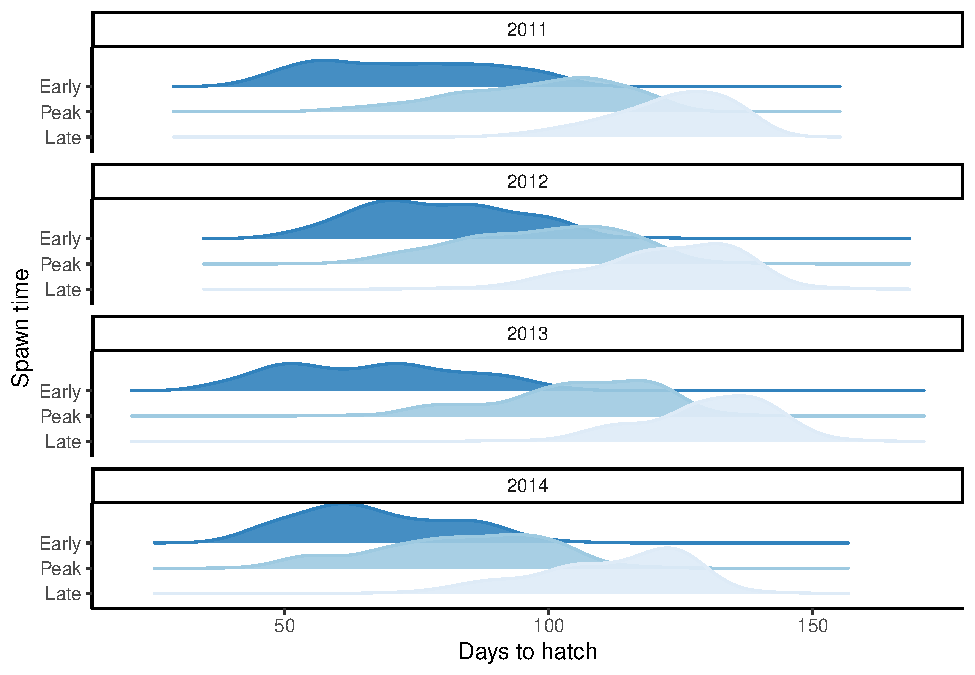
\includegraphics{paper_files/figure-latex/unnamed-chunk-19-1.pdf}
\caption{Densities of predicted days to hatch for Bull Trout for 139
putative spawning locations across Idaho for four years of shared
temperature data. Early spawning considers if a parent spawned September
1, Peak-September 15, and Late-September 30.}
\end{figure}

\section{Discussion}\label{discussion}

With \textbf{hatchR} we present a software ecosystem that bridges the
analytical gap of predicting developmental phenology for wild fishes and
develops a formal framework for applying effective value models from
user-provided parameterizations. To do so, the software is bundled in
two forms, a fully customizable R package, especially useful for running
repetitive analyses and a graphical-user-interface designed for ease of
use and tasks that may only run once or a handful of times. Both
applications allows users to import their data, run basic data checks,
and apply historic model parameterizations for salmonids or create their
own species- or population specific parameterization. Additionally, we
provide substantial documentation on the \textbf{hatchR} website
(\url{https://bmait101.github.io/hatchR/}) to walk users through basic
to advanced applications of programmatic platform.

In the application of using effective value models \textbf{hatchR} and
the user make some key assumptions. Particularly, numerous studies have
indicated that stressful environmental conditions can cue fish to
prematurely hatch or emerge from their environment. These include water
quality like dissolved oxygen, pH, or salinity, pathogens, and even
mechanical agitation (reviewed in Quinn (2018) and Cowan et al. (2024)).
Moreover, while the \textbf{hatchR} provides point estimates for
developmental phenology, spawning and developmental within populations
of fishes both occur as distributions as opposed single events Mason
(1976) and we encourage users to either predict phenology using early,
peak, and late frameworks (\emph{e.g.}, 5th, 50th, and 95th quantiles)
or with real or modeled distributions. Another factor that could bias
estimates from these models is that temperatures used from sensors don't
reflect the geomoprhic properties in the environment where eggs are
developing such that they may be too cold or warm Geist et al. (2002).

To date, the application of the effective value framework has largely
focused using species-specific models to predict phenology in wild
environments (see Adelfio et al. (2024), Austin et al. (2019)). However,
we emphasize that the statistical relationships at the basis of these
models are fundamentally reaction norms, meaning that both the intercept
and slope of the responses of fishes to temperature are reflective of
family- or population-level genetic variation, genetic x environment
responses, or may be indicative of phylogenetic differences among
species (West-Eberhard (2003)). For instance, while Sparks et al. (2017)
did not find differences in the rates of development between the focal
populations of their study, they did observe family-level genetic x
environment interactions across different thermal regimes. Similarly,
when they reparameterized their models using fish from western Alaska,
they found differences in both the slope and intercept of the model
relative to the original parameterization from Beacham \& Murray (1990),
notably derived from multiple Canadian stocks. The western Alaskan fish
generally developed more slowly than their southerly counterparts,
consistent with cogradient variation (Conover, Duffy, \& Hice (2009),
Sparks, Kraft, Blackstone, McNickle, \& Christie (2022)). In this sense,
we encourage users not to only think about the end points of these
models (days to development) but also how the statistical relationships
they are premised on inform our understanding of micro- and and
macro-evolutionary processes.

\textbf{BRYAN check the below}

The models presented in \textbf{hatchR} can be further customized in
multiple ways beyond the use-cases provided above. For instance, while
our models are fit to predict hatch or emergence timing, they could be
used to predict other developmental stages prior to the initation of
external feeding like eye-up or other embryological developmental stages
(Velsen (1980)) or \textbf{Some example from a non-salmonid, maybe
initiation of pelagic-larval or riverine current dispersal}.
Additionally, while \texttt{fit\_model()} relies on non-linear modeling
platform, \texttt{predict\_phenology()} only requires users to pass a
model expression, so if users preferred a different model fit than the
non-linear option provided (as long as it integrates daily temperature),
they could pass a different expression into
\texttt{predict\_phenology()} for additional customization. Finally,
while \textbf{hatchR} was designed specifically for fishes, we expect
other poikilothermic organisms such as reptiles, amphibians, or
invertebrates would develop in accordance with the power law and these
developmental models could be extended to other organisms beyond fishes.

\section{Acknowledgements}\label{acknowledgements}

We thank Laura Koller for her help designing the \textbf{hatchR} logo.
Dan Isaak provided useful discussion about model development and
temperature datasets.

The views expressed in this manuscript are those of the authors and do
not necessarily represent the views or policies of USFS or USFWS. Any
mention of trade names, products, or services does not imply an
endorsement by the U.S. government, USFS, or USFWS. USFS and USFWS do
not endorse any commercial products, services or enterprises.

\section*{References}\label{references}
\addcontentsline{toc}{section}{References}

\phantomsection\label{refs}
\begin{CSLReferences}{1}{0}
\bibitem[\citeproctext]{ref-adelfio2019}
Adelfio, L. A., Wondzell, S. M., Mantua, N. J., \& Reeves, G. H. (2019).
Warm winters reduce landscape-scale variability in the duration of egg
incubation for coho salmon (oncorhynchus kisutch) on the copper river
delta, alaska. \emph{Canadian Journal of Fisheries and Aquatic
Sciences}, \emph{76}(8), 1362--1375.
doi:\href{https://doi.org/10.1139/cjfas-2018-0152}{10.1139/cjfas-2018-0152}

\bibitem[\citeproctext]{ref-adelfio2024}
Adelfio, L. A., Wondzell, S. M., Mantua, N. J., \& Reeves, G. H. (2024).
Expanded, compressed, or equal? Interactions between spawning window and
stream thermal regime generate three responses in modeled juvenile
emergence for pacific salmon. \emph{Canadian Journal of Fisheries and
Aquatic Sciences}.
doi:\href{https://doi.org/10.1139/cjfas-2023-0238}{10.1139/cjfas-2023-0238}

\bibitem[\citeproctext]{ref-alderdice1978}
Alderdice, D. F., \& Velsen, F. P. J. (1978). Relation between
temperature and incubation time for eggs of chinook salmon (oncorhynchus
tshawytscha). \emph{Journal of the Fisheries Research Board of Canada},
\emph{35}(1), 69--75.
doi:\href{https://doi.org/10.1139/f78-010}{10.1139/f78-010}

\bibitem[\citeproctext]{ref-austin2019}
Austin, C. S., Essington, T. E., \& Quinn, T. P. (2019). Spawning and
emergence phenology of bull trout Salvelinus confluentus under differing
thermal regimes. \emph{Journal of Fish Biology}, \emph{94}(1), 191--195.
doi:\href{https://doi.org/10.1111/jfb.13864}{10.1111/jfb.13864}

\bibitem[\citeproctext]{ref-beacham1990}
Beacham, T. D., \& Murray, C. B. (1990). Temperature, egg size, and
development of embryos and alevins of five species of pacific salmon: A
comparative analysis. \emph{Transactions of the American Fisheries
Society}, \emph{119}(6), 927--945.
doi:\href{https://doi.org/10.1577/1548-8659(1990)119\%3C0927:TESADO\%3E2.3.CO;2}{10.1577/1548-8659(1990)119\textless0927:TESADO\textgreater2.3.CO;2}

\bibitem[\citeproctext]{ref-chang2024}
Chang, W., Cheng, J., Allaire, J. J., Sievert, C., Schloerke, B., Xie,
Y., Allen, J., et al. (2024). \emph{Shiny: Web application framework for
r}. Retrieved from
\url{https://cran.r-project.org/web/packages/shiny/index.html}

\bibitem[\citeproctext]{ref-conover2009}
Conover, D. O., Duffy, T. A., \& Hice, L. A. (2009). The Covariance
between Genetic and Environmental Influences across Ecological
Gradients. \emph{Annals of the New York Academy of Sciences},
\emph{1168}(1), 100--129.
doi:\href{https://doi.org/10.1111/j.1749-6632.2009.04575.x}{10.1111/j.1749-6632.2009.04575.x}

\bibitem[\citeproctext]{ref-cowan2024}
Cowan, Z.-L., Green, L., Clark, T. D., Blewett, T. A., De Bonville, J.,
Gagnon, T., Hoots, E., et al. (2024). Global change and premature
hatching of aquatic embryos. \emph{Global Change Biology}, \emph{30}(9),
e17488. doi:\href{https://doi.org/10.1111/gcb.17488}{10.1111/gcb.17488}

\bibitem[\citeproctext]{ref-geist2002}
Geist, D. R., Hanrahan, T. P., Arntzen, E. V., McMichael, G. A., Murray,
C. J., \& Chien, Y.-J. (2002). Physicochemical Characteristics of the
Hyporheic Zone Affect Redd Site Selection by Chum Salmon and Fall
Chinook Salmon in the Columbia River. \emph{North American Journal of
Fisheries Management}, \emph{22}(4), 1077--1085.
doi:\href{https://doi.org/10.1577/1548-8675(2002)022\%3C1077:PCOTHZ\%3E2.0.CO;2}{10.1577/1548-8675(2002)022\textless1077:PCOTHZ\textgreater2.0.CO;2}

\bibitem[\citeproctext]{ref-isaak2018}
Isaak, D. J., Luce, C. H., Chandler, G. L., Horan, D. L., \& Wollrab, S.
P. (2018). Principal components of thermal regimes in mountain river
networks. \emph{Hydrology and Earth System Sciences}, \emph{22}(12),
6225--6240.
doi:\href{https://doi.org/10.5194/hess-22-6225-2018}{10.5194/hess-22-6225-2018}

\bibitem[\citeproctext]{ref-isaak2015}
Isaak, D. J., Young, M. K., Nagel, D. E., Horan, D. L., \& Groce, M. C.
(2015). The cold-water climate shield: delineating refugia for
preserving salmonid fishes through the 21st century. \emph{Global Change
Biology}, \emph{21}(7), 2540--2553.
doi:\href{https://doi.org/10.1111/gcb.12879}{10.1111/gcb.12879}

\bibitem[\citeproctext]{ref-kaylor2021}
Kaylor, M. J., Justice, C., Armstrong, J. B., Staton, B. A., Burns, L.
A., Sedell, E., \& White, S. M. (2021). Temperature, emergence phenology
and consumption drive seasonal shifts in fish growth and production
across riverscapes. \emph{Journal of Animal Ecology}, \emph{90}(7),
1727--1741.
doi:\href{https://doi.org/10.1111/1365-2656.13491}{10.1111/1365-2656.13491}

\bibitem[\citeproctext]{ref-mason1976}
Mason, J. (1976). Some features of coho salmon, oncorhynchus kisutch,
fry emerging from simulated redds and concurrent changes in
photobehavior. \emph{Fish. Bull}, \emph{74}(1), 167--175.

\bibitem[\citeproctext]{ref-mcphail1979}
McPhail, J., \& Murray, C. (1979). \emph{The early life-history and
ecology of dolly varden (salvelimus malma) in the upper arrow lakes}.
Nelson, BC, Canada.

\bibitem[\citeproctext]{ref-nolfi2024}
Nolfi, D., Melbihess, T., Fisher, S., \& Ellis, L. (2024). 5-Year
Statuse Review Coterminous United States Population of Bull Trout
(Salvelinus confluentus).

\bibitem[\citeproctext]{ref-quinn2018}
Quinn, T. P. (2018). \emph{The Behavior and Ecology of Pacific Salmon
and Trout}. University of Washington Press.

\bibitem[\citeproctext]{ref-r:ther}
R: The r project for statistical computing. (n.d.). Retrieved from
\url{https://www.r-project.org/}

\bibitem[\citeproctext]{ref-siegel2023}
Siegel, J. E., Fullerton, A. H., FitzGerald, A. M., Holzer, D., \&
Jordan, C. E. (2023). Daily stream temperature predictions for
free-flowing streams in the Pacific Northwest, USA. \emph{PLOS Water},
\emph{2}(8), e0000119.
doi:\href{https://doi.org/10.1371/journal.pwat.0000119}{10.1371/journal.pwat.0000119}

\bibitem[\citeproctext]{ref-small2001}
Small, B. C., \& Bates, T. D. (2001). Effect of Low-Temperature
Incubation of Channel Catfish Ictalurus punctatus Eggs on Development,
Survival, and Growth. \emph{Journal of the World Aquaculture Society},
\emph{32}(2), 189--194.
doi:\href{https://doi.org/10.1111/j.1749-7345.2001.tb01094.x}{10.1111/j.1749-7345.2001.tb01094.x}

\bibitem[\citeproctext]{ref-smith2005}
Smith, K. M., \& King, D. K. (2005). Dynamics and extent of larval lake
sturgeon Acipenser fulvescens drift in the Upper Black River, Michigan.
\emph{Journal of Applied Ichthyology}, \emph{21}(3), 161--168.
doi:\href{https://doi.org/10.1111/j.1439-0426.2005.00623.x}{10.1111/j.1439-0426.2005.00623.x}

\bibitem[\citeproctext]{ref-sparks2019}
Sparks, M. M., Falke, J. A., Quinn, T. P., Adkison, M. D., Schindler, D.
E., Bartz, K., Young, D., et al. (2019). Influences of spawning timing,
water temperature, and climatic warming on early life history phenology
in western alaska sockeye salmon. \emph{Canadian Journal of Fisheries
and Aquatic Sciences}, \emph{76}(1), 123--135.
doi:\href{https://doi.org/10.1139/cjfas-2017-0468}{10.1139/cjfas-2017-0468}

\bibitem[\citeproctext]{ref-sparks2022}
Sparks, M. M., Kraft, J. C., Blackstone, K. M. S., McNickle, G. G., \&
Christie, M. R. (2022). Large genetic divergence underpins cryptic local
adaptation across ecological and evolutionary gradients.
\emph{Proceedings of the Royal Society B: Biological Sciences},
\emph{289}(1984), 20221472.
doi:\href{https://doi.org/10.1098/rspb.2022.1472}{10.1098/rspb.2022.1472}

\bibitem[\citeproctext]{ref-sparks2017}
Sparks, M. M., Westley, P. A. H., Falke, J. A., \& Quinn, T. P. (2017).
Thermal adaptation and phenotypic plasticity in a warming world:
Insights from common garden experiments on Alaskan sockeye salmon.
\emph{Global Change Biology}, \emph{23}(12), 5203--5217.
doi:\href{https://doi.org/10.1111/gcb.13782}{10.1111/gcb.13782}

\bibitem[\citeproctext]{ref-velsen1980}
Velsen, F. P. J. (1980). Embryonic Development in Eggs of Sockeye Salmon
Oncorhynchus nerka. \emph{Canadian Special Publication of Fisheries and
Aquatic Sciences}, (49).

\bibitem[\citeproctext]{ref-webster1948}
Webster, D. A. (1948). Relation of temperature to survival and
incubation of the eggs of smallmouth bass (micropterus dolomieu).
\emph{Transactions of the American Fisheries Society}, \emph{75}(1),
43--47.
doi:\href{https://doi.org/10.1577/1548-8659(1945)75\%5B43:ROTTSA\%5D2.0.CO;2}{10.1577/1548-8659(1945)75{[}43:ROTTSA{]}2.0.CO;2}

\bibitem[\citeproctext]{ref-west-eberhard2003}
West-Eberhard, M. J. (2003). \emph{Developmental Plasticity and
Evolution}. Oxford University Press.

\end{CSLReferences}

\end{document}
